\documentclass[a4paper,12pt]{article}
\usepackage[left=2cm,right=1cm,top=2cm,bottom=2cm]{geometry}
\usepackage{amsmath}
\usepackage{listings}
\usepackage{latexsym}
\usepackage{amsmath}
\usepackage{amssymb}
\usepackage{graphicx}
\usepackage{wrapfig}
\pagestyle{plain}
\usepackage{fancybox}
\usepackage{bm}
\usepackage[utf8]{inputenc}
\usepackage[russian]{babel}
\usepackage{floatrow}
\usepackage{pdfpages}
\usepackage{ragged2e}
\usepackage{algorithm}
\usepackage{algpseudocode}
\documentclass{article}
\usepackage[T2A]{fontenc}
\usepackage[utf8]{inputenc}
\usepackage[english, russian]{babel}
\justifying
\usepackage[inkscapeformat=png]{svg}
\usepackage[pageanchor]{hyperref}
\algblock[BLOCK]{parfor}{endparfor}

\begin{document}
\tableofcontents
\hyperpage{}

\newpage
\section{Введение} 
Метод Лаггера часто используется как практически беспроигрышный вариант во многих случаях, когда нужно быстро и сравнительно надёжно вычислить корни многочлена. Однако есть случаи, когда метод сойтись не может, либо встречает на пути к достаточному приближению препятствия. Алгоритм сумм степеней (Sums of Powers Algorithm) позволяет подстраховать метод Лаггера в этих случаях, вычисляя корни с достаточной точностью, и самое главное, с полной надёжностью. Алгоритм LaSPA (Laguerre SPA) является быстрым, и, в то же время, чрезвычайно надёжным методом для вычисления корней многочленов.
\newpage
\section{Обзор и доказательная база метода}
\subsection{Основные определения и обозначения}
Пусть есть многочлен 
\begin{equation}
    p(z)=\sum_{i=0}^m{a_iz^i}, a_i \in \mathbb{C}, i \in \{1,\dots,m\}
\end{equation}
Здесь $a_i$ - коэффициенты, $m+1$ - степень многочлена. \\
Для определённости сразу скажем, что в общем случае, нас интересуют многочлены степени больше 3. Если какие-то части алгоритма встречаются с многочленами степеней ниже, они пользуются аналитической формулой для квадратного или линейного многочлена. 
\subsection{Критерий сходимости и оценка ошибки}
Для любого простого (не кратного) корня $\rho$ многочлена $p(z)$ с помощью разложения в ряд Тейлора можно доказать, что метод Лаггера сходится кубически к пределу $\rho$ вне зависимости от близости начального приближения. Однако не была известна окрестность этого корня (насколько малое расстояние необходимо для этого условия). В следующей теореме мы устанавливаем, что для каждого простого корня $\rho$ существует диск с центром в точке $\rho$, в котором любое начальное приближение обеспечивает гарантированную сходимость метода.
\\
\textbf{Теорема 1.} Пусть $p(z)$ - нормализованный многочлен степени больше 3, $P={\rho_1, \dots, \rho_l}$ - множество корней. Тогда для схемы Лаггера действует следующее: \\\\
Если есть простой корень $\rho \in P$ такой, что выполняется условие
\begin{equation}
    |u_0-\rho| \leq \frac{1}{2m-1}min \{ |\sigma - \rho|, \sigma \in P \textbackslash \{ \rho \}\}
\end{equation}
Тогда последовательность Лаггера $L_p(u_0)$ сходится к пределу $\rho$, выполняется
\begin{equation}
    |u_n-\rho| < \lambda ^ n |u_0-\rho|,
\end{equation}
 $\text{ где } \lambda = \frac{15}{16} \text{ } \forall n \in \mathbb{N}$ \\
Таким образом, обеспечивается, по крайней мере, линейная сходимость на всех дисках простых корней. \\\\
\textbf{Теорема 2.} Пусть $p(z)$ - нормализованный многочлен степени больше 3. Тогда 
\begin{equation}
    k(0)=min\{k \in J_m|a_k \noteq 0\}
\end{equation}
и 
\begin{equation}
    q_0=m(k(0)\cdot a_{k(0)})^{-1}
\end{equation}
Пусть $k(s)$ и $q_s$ известны для $s=max\{0, n-m\},\dots,n-1$. Тогда $k(n)$ и $q_n$ можно вычислить следующим образом: \\
Для $s=max\{0, n-m\},\dots,n-1$ и для $t \in J_m$, возьмём \\
\begin{equation}
    \begin{cases}
      q_s, когда s>0, q_s \noteq 0, \\
      1, когда s>0, q_s=0, \\
      t(k(0)a_{k(0)}^{-1}, когда s=0,
    \end{cases}\,.
\begin{cases}
      q_s, когда s>0, q_s \noteq 0, \\
      1, когда s>0, q_s=0, \\
      t(k(0)a_{k(0)}^{-1}, когда s=0,
    \end{cases}\,.
\end{equation}
\newpage
\subsection{Точки старта}
Требуется показать области выполнения неравенства:
\begin{equation} \label{eq:1}
    |u_0-\rho| \leq \frac{1}{2m-1}min \{ |\sigma - \rho|\sigma \in P \textbackslash \{ \rho \} \}
\end{equation}
В большинстве случаев выгодно взять арифметическое среднее корней: \\
$\alpha=-\frac{1}{m}a_{m-1}a^{-1}_m$. Если для $\alpha$ верно $q(\alpha)+s(\alpha)r(\alpha) \neq 0$ и оно лежит в квадрате, то это оптимальная точка старта.
Возможные точки старта алгоритма могут быть разделены на 4 класса:
\begin{enumerate}
    \item внутренние точки - в них обычный алгоритм Лагерра сойдётся гарантированно за определённо взятое количество шагов;
    \item граничные точки, или точки шага - возможно, потребуется больше итераций, однако, алгоритм сойдётся;
    \item циклические точки - генерируют циклические последовательности Лаггера;
    \item сингулярные точки - нули производной многочлена, как начальное приближение не используется из-за мгновенного выхода алгоритма в бесконечность.
\end{enumerate}
Приведём свойства этих точек и областей, которые они образуют на комплексной плоскости, рассматриваемой на предмет выполнения неравенства (\ref{eq:1}): \\
\begin{itemize}
    \item если у многочлена нет точек сингулярности, существует такое число $S_p$, что стартовые точки одного типа с модулем больше $S_p$ формируют негораниченные просто связные области;
    \item если $\zeta$ - точка сингулярности или циклическая точка, то для любого номера $N \in \mathbb{N}$ существует такой диск $\delta_N$ с центром в $\zeta$, что все количества шагов для траекторий с начальной точкой $u_0 \in \delta_N \textbackslash {\zeta}$ больше $N$. Иначе говоря, выбраться алгоритмом Лагерра из точек цикла и сингулярности невозможно, каждая итерация приводит к увеличению количества необходимых шагов;
    \item только циклические и сингулярные точки являются изолированными, то есть, их окрестность пересекается с множеством выполнения неравенства только в них;
    \item Граничная кривая каждой области ступеньки полностью или частично принадлежит один из соседних районов
\end{itemize}
Теперь рассмотрим многочлен с корнями $$[1.6-0.55j, -0.39+0.03j, -2.32+2.17j, 0.2-1.06j, -0.02-0.27j]$$ Это многочлен 5 степени $$(0.306917 - 0.531751 i)-(1.61433 + 2.57707 i) x-$$ $$-(6.2503 + 1.40811 i) x^2 - (0.5818 - 5.8351 i) x^3 + (0.93 - 0.32 i) x^4 + x^5$$
График корней на комплексной плоскости:
\begin{figure}[hbt!]
    \centering
    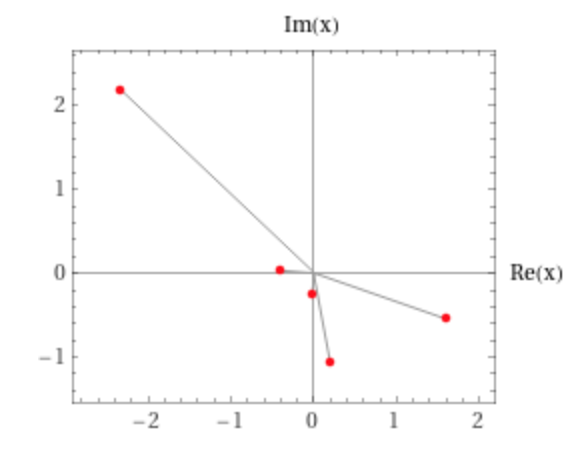
\includegraphics{images/roots_on_a_plane.png}
    \caption{Корни многочлена на комплексной плоскости}
    \label{fig:enter-label}
\end{figure}
Визуализируем все типы точек на графике:
\newpage
\begin{figure}[hbt!]
    \centering
    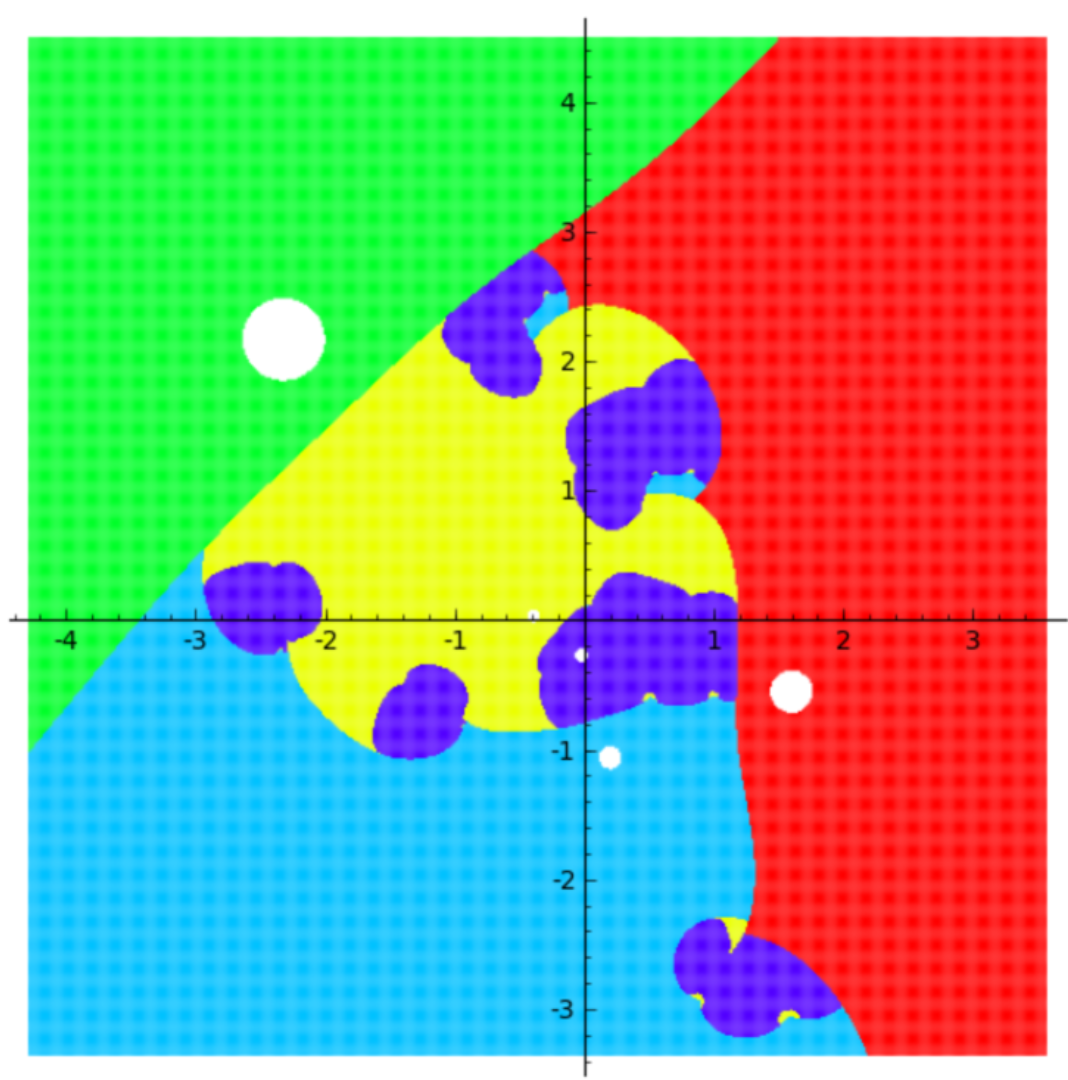
\includegraphics[width=0.75\linewidth]{images/fig1.png}
    \caption{Безопасные (белым) и предельные зоны}
\end{figure}
\newpage
\begin{figure}[hbt!]
    \centering
    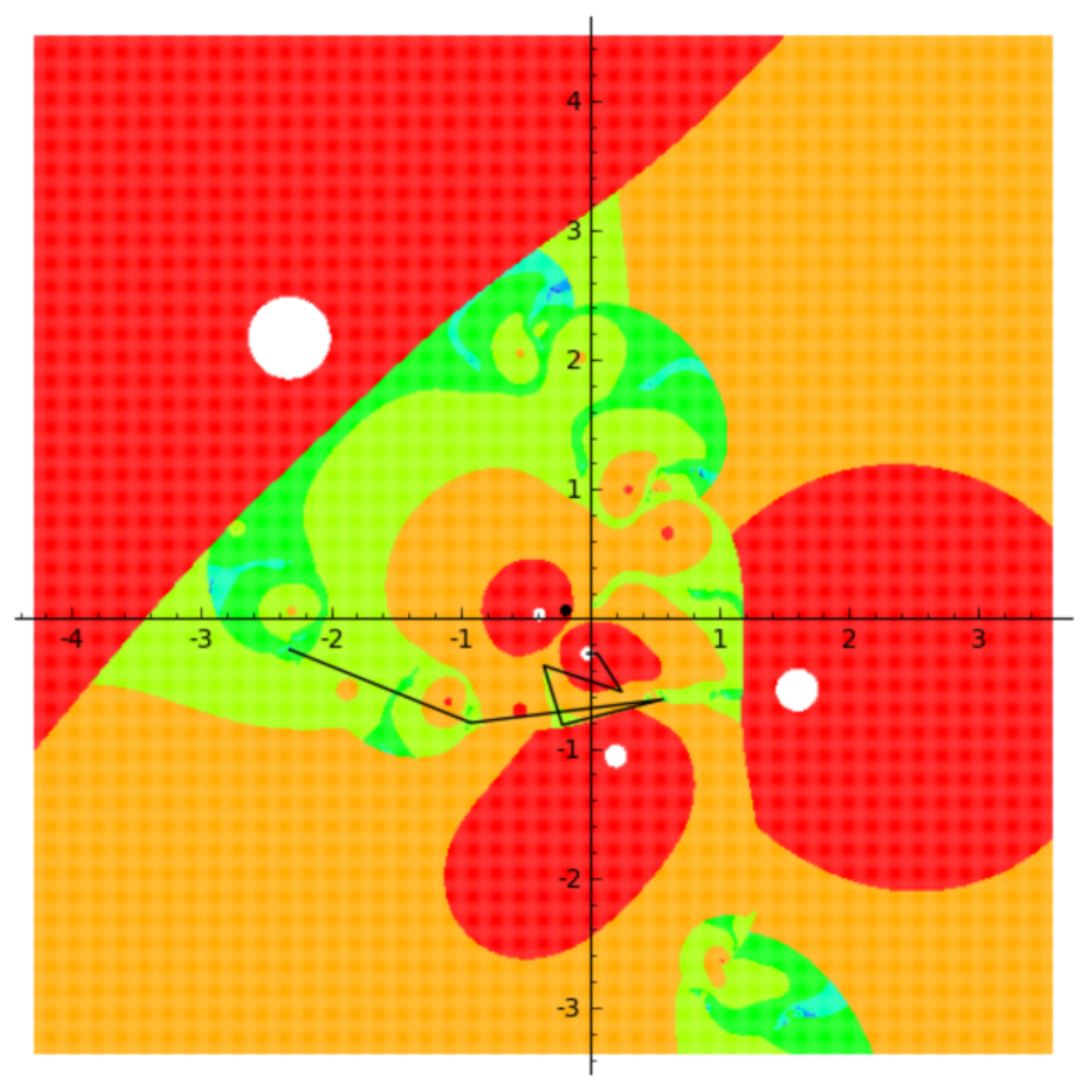
\includegraphics[width=0.75\linewidth]{images/fig2.png}
    \caption{Безопасные зоны, области шага, траектория наибольшего количества шагов, среднее арифметическое корней (чёрным цветом)}
    \label{fig:enter-label}
\end{figure}
\newpage
\subsection{SPA - Sums of Powers Algorithm}
Краткое описание алгоритма:
\begin{enumerate}
    \item Производится попытка выполнения обычного метода Лаггера. Для улучшения скорости сходимости стоит выбрать наиболее оптимальное начальное приближение без учёта остальных свойств многочлена - среднее арифметическое корней. Его можно найти по формуле $-\frac{1}{m}a_{m+1}a_m^{-1}$.
    \item Если количество итераций, необходимое для получения результата, достаточного по точности, даёт неудовлетворительную точность, применяем алгоритм SPA непосредственно.
    \item Из пункта 1 получаем значения приближений корней. Как правило, они бывают уже достаточно близкие к настоящим значениям. Расставляем их по возрастанию их модуля: $0 < |z_1| < |z_2| < \dots < |z_k|$. Это необходимо, чтобы упорядочить их по радиусу от точки отсчёта.
    \item Используем для полученных приближений метод наименьших кругов. Это должно получить достаточные по заданной точности $\epsilon$ приближения корней для подавляющего числа многочленов (по крайней мере, на практике не встречалось иного)
    \item В так называемом \textit{экстремальном случае} используется метод колец Турана. Он гарантированно находит кольцо, в котором находится искомый корень, причём кольцо достаточно тонкое, чтобы удовлетворять заданной точности.
\end{enumerate}
Теперь остановимся на каждом шаге поподробнее:
\begin{enumerate}
    \item Вначале используется обычный метод Лаггера. Для большинства многочленов ожидается, что он сойдётся - нулями около точек сингулярности и циклов обладают не так много многочленов, как показывает практика. Для улучшения скорости сходимости стоит выбрать наиболее оптимальное начальное приближение без учёта остальных свойств многочлена - среднее арифметическое корней. Его можно найти по формуле $-\frac{1}{m}a_{m+1}a_m^{-1}$.
    \item Если количество итераций, необходимое для получения результата, достаточного по точности, даёт неудовлетворительную точность, применяем алгоритм SPA непосредственно.
    \item Из пункта 1 получаем значения приближений корней. Как правило, они бывают уже достаточно близкие к настоящим значениям. Расставляем их по возрастанию их модуля: $0 < |z_1| < |z_2| < \dots < |z_k|$. Это необходимо, чтобы упорядочить их по радиусу от точки отсчёта.
    % \item Вычисляем необходимое количество итераций для получения результата в виде достаточного приближения корня. Это делается по следующей формуле:
    % \begin{equation}
    %     n_{\epsilon}=[(log \kappa^{-1})^{-1} log(4mb \epsilon^{-1})]+1
    % \end{equation}
    % Путём проверки на практике было получено, что $n_{\epsilon}=4$ - наилучший параметр для наших целей.
    % \item используя метод Бернулли, получаем суммы степеней нужных нам корней
    \item Начинаем алгоритм наименьших кругов. Для начала скажем, что все корни многочлена $p(z)$ образуют на аналитическом пространстве $\{(x,y,w)\in \mathbb{R}^{3}|w=|p(x+iy)|^{2}$\}. Следовательно, пользуясь методом наименьших кругов, будем получать сдвиги многочленов близкие к кругу минимальных расстояний - минимальному кругу без точек минимума. \\
    Берём функцию 
    \begin{equation}
        \pi_r:=(t\xrightarrow{}|p(rcost+irsint)|^2,t\in [0,2\pi])
    \end{equation}
    получаем разложение в ряд Фурье: \\
\[
\pi_r(t)-f_0=\sum_{k=1}^{m} (f_k2cos(kt)+g_k2cos(\frac{3\pi}{2}+kt))
\]
затем получаем значение производной
\[
\pi_r(t)^{'}=\sum_{k=1}^{m} (kg_k2cos(kt)-kf_k2cos(\frac{3\pi}{2}+kt))
\]
в равноудалённых точках $t$ по таблице значений $2cos(\pi n/(3N))$, где $n=0,\dots,6N-1$, получаемыми рекурсивно:
\[
2cos((n+2)\Delta)=(2cos\Delta)(2cos((n+1)\Delta))-2cos(n\Delta)
\]
где $n=0,\dots,3N-1$, $\Delta:=\frac{\pi}{3N}$.
Далее вычисляются точки $x_j, j \in \{1,\dots,e\}$, в которых $\pi_r^{'}(x_j)\leq0$, но $\pi_r^{'}(x_j+\Delta)>0$. В этих точках вычисляется точка минимума: $rcosx_j+ircos(3\pi/2+x_j), j=\{1,\dots,e\}$. Эти точки аппроксимируют локальный минимум. Назовём их точками минимума. Их можно использовать как смещение для многочлена.
    \item Вычислим для многочлена диаметр Лаггера. Если для всех корней он превышает заданную точность, то выходим на пункт 6. Иначе берём каждый, для которого диаметр Лаггера меньше $\epsilon$, то есть, для которого выполняется условие сходимости, как достаточное приближение корня. Будем называть минимальным кругом множество точек круга с минимальным расстоянием в совокупности с минимальным точками $x_j$. Так как корни близки к кругу, стоит снизить шаг алгоритма, приближающего корни (Бернулли) до 2.0.
    \item Пусть найдена точка с минимальным диаметром Лаггера (то есть, максимально ограничивающая приближение корня). Смещаем многочлен на неё, берём радиус минимального круга $r_1$ для смещённого многочлена. Если $r_1 < 0.3r$, то идём дальше, строим минимальный круг для полученного. Это называется цепочка минимальных кругов.
    \item Если для двоих кругов подряд не выполнится $r_1 < 0.3r$, возникает особая ситуация, требующая заменить минимальный круг кругом Турана. Это множество следующего вида:
\[
\mathcal{T}(\xi):=\{z\in\mathbb{C}||z-\xi|=\sigma_{16m}\}
\]
Его радиус равен $r^{'}=\sigma_{16m}$, и для него верно $0.9r^{'}<0.2^\frac{1}{16}r^{'}<|z_1|<r^{'}$. \\
Получается кольцо Турана, покрываемое 12 дисками следующего вида: 
\begin{equation}
    \{z \in \mathbb{C}||z-\xi_j|\leq \nu r^{'}\}
\end{equation}
где
\begin{align}
    \xi_j:=(19r{'}/20)cos(j\pi/6)+isin(j\pi/6), j=0,\dots,11,  \\
    \nu=\sqrt{1/400+(19/5)sin^{2}(\pi/24)}
    \end{align}
$z_1$ находится в одном из этих дисков. \\
\end{enumerate}
\newpage
% \subsection{Критерий остановки}
% Критерий остановки выражается через количество итераций и теорему 1. \\
% \textbf{Теорема 1.} Пусть $z_1,\dots,z_k$ - комплексные числа такие, что $k \in \mathbb{N} \textbackslash \{1\} и z_g \neq z_h для g,h \in \{1,\dots,m\} \text{, при} \\ \text{ этом } |z_1|<|z_2| \text{ и } |z_1| \leq b$, где $b$ - выбираемый параметр. Если $\epsilon \text{ и } \kappa$ - действительные числа с ограничениями $0<\epsilon \leq 2b$ и $|z_1/z_2|\leq\kappa<1$, тогда условие $|q_n-z_1|<\epsilon$ сохраняется для каждого $n \in \mathbb{N}_0$, помимо этого:
% \[
% n \geq  [(log\kappa^{-1})^{-1}log(4mb\epsilon^{-1})]+1
% \]
% Из большого числа тестов стало известно, что наилучшее значение для $n$ это 3.0. \\
% Для случаев, когда $|z_2| \geq 1.4|z_1|$ данное число итераций даст достаточную точность. Однако, даже если оно не выполняется, можно получить достаточное приближение корней с помощью метода минимума из части \ref{2.7}.
% Затем это слагаемое выбирается равным двум, что соответствует $|z_2| \geq 1.65|z_1|$. \\
% \end{enumerate}

% \[
% \mathcal{T}(\xi):=\{z\in\mathbb{C}||z-\xi|=\sigma_{16m}\}
% \]
% Его радиус равен $r^{'}=\sigma_{16m}$, и для него верно $0.9r^{'}<0.2^\frac{1}{16}r^{'}<|z_1|<r^{'}$. Получается кольцо Турана, покрываемое 12 дисками следующего вида: $\{z \in \mathbb{C}||z-\xi_j|\leq \nu r^{'}\}$, где $\xi_j:=(19r{'}/20)cos(j\pi/6)+isin(j\pi/6), j=0,\dots,11, \nu=\sqrt{1/400+(19/5)sin^{2}(\pi/24)}$. $z_1$ находится в одном из этих дисков. \\
% \newpage
% \subsection{Критерий остановки}
% Критерий остановки выражается через количество итераций и теорему 1. \\
% \textbf{Теорема 1.} Пусть $z_1,\dots,z_k$ - комплексные числа такие, что $k \in \mathbb{N} \textbackslash \{1\} и z_g \neq z_h для g,h \in \{1,\dots,m\} \text{, при} \\ \text{ этом } |z_1|<|z_2| \text{ и } |z_1| \leq b$, где $b$ - выбираемый параметр. Если $\epsilon \text{ и } \kappa$ - действительные числа с ограничениями $0<\epsilon \leq 2b$ и $|z_1/z_2|\leq\kappa<1$, тогда условие $|q_n-z_1|<\epsilon$ сохраняется для каждого $n \in \mathbb{N}_0$, помимо этого:
% \[
% n \geq  [(log\kappa^{-1})^{-1}log(4mb\epsilon^{-1})]+1
% \]
% Из большого числа тестов стало известно, что наилучшее значение для $n$ это 3.0. \\
% Для случаев, когда $|z_2| \geq 1.4|z_1|$ данное число итераций даст достаточную точность. Однако, даже если оно не выполняется, можно получить достаточное приближение корней с помощью метода минимума из части \ref{2.7}.
% Затем это слагаемое выбирается равным двум, что соответствует $|z_2| \geq 1.65|z_1|$. \\
% \textbf{Теорема 3.}
% Если приближение корня $u \in \mathbb{C} - (Z \cap Z_1)$, тогда для каждого круга, проходящего через $u$ и $h_m(u)$ есть два варианта:
% \begin{itemize}
%     \item есть элементы $Z$ внутри и снаружи круга
%     \item все числа из $Z$ лежат на круге
% \end{itemize}
% Диск Лаггера для точки $u$ имеет радиус меньше $m|u-z_j|$, если $u$ достаточно близко к $z_j \in \mathcal{Z}$: \\
% \textbf{Теорема 4.} Пусть $p(z)$ - многочлен с количеством различных корней больше или равным 2. Если $z_j \in \mathcal{Z}$, то
% \[
% |u-z_j|<m\frac{|p(u)|}{|p^{'}(u)|}\leq\frac{2m-1}{2m_j-1}|u-z_j|
% \]
% и равенство $\mathcal{L}_u \cap \mathcal{Z}=\{z_j\}$ сохраняется для каждого $u \in \mathbb{C}$ и $0<|u-z_j|\leq\mu_j/(2m)$. \\
% Из этого получаем критерий остановки для первых двух стадий SPA: \\
% Так как ранее указанное количество шагов, указанное в теореме 1, покрывает большую часть коэффициентов сходимости $|z_1/z_2|$, рекомендуется сделать предпроверку вместо проверки условия сходимости $m|p(q_n)/p^{'}(q_n)|\leq\epsilon$ из теоремы 4 на каждой итерации.
% \newpage
% \subsection{Границы ошибки}
% Закрытый диск
% \[
% \mathcal{L}_u=\mathcal{L}_u(p):=\{w \in \mathbb{C}||w-h_{m/2}(u)|\leq |u-h_{m/2}|\}
% \]
% называется диском Лаггера для приближения $u$, гарантированно содержит, как минимум, один корень $p$. \\
% \textbf{}
% Из данной теоремы следует, что радиус диска Лаггера $\mathcal{L}_u$ меньше чем $m|u-z_j|$, если $u$ достаточно близка к $z_j \in \mayhcal{Z}$.
% \newpage
% \subsection{Метод минимума}
% \label{2.7}
% Метод минимума применяется, когда первые $n_\epsilon$ членов последовательности Лаггера (или Бернулли) недостаточно аппроксимируют $z_1$. \\
% \textbf{Теорема 6.} Пусть $z_1,\dots,z_k$ - множество комплексных корней многочлена, $h(n)$ - рекуррентное соотношение с условием: \\
% \begin{cases}
%     h(0):=k(0) \\
%     h(j+1):=k(h(j)) \forall j \in \mathbb{N}_0
% \end{cases}
% Если $c_n:=|ms^{-1}_{h(n)}|^{1/h(n)}$ для $n \in \mathbb{N}_0$, то $|z_1|$ - предел последовательности $(\sigma_n)_n$, где \\
% \[
% \sigma_n:=min\{s \in \mathbb{R}|\exists j \in \mathbb{N}_0 : \leq max\{h(0),n\} \text{и} s=c_j\}
% \]
% для $n \in \mathbb{N}_0$, которое состоит из "последовательных минимумов" $(c_n)_n$. Помимо этого, \\
% \[
% (5^{-2})^{-\nu}\sigma_{m2^{\nu}}<|z_1|\leq \sigma_{m2^{\nu}} \text{ для каждого } \nu \in \mathbb{N}_0
% \]
% Степени $c_n^{h(n)}$ могут быть вычислены рекурсивно по следующей формуле: \\
% \[
% c_0^{h(0)}=|q_0|, c_{n+1}^{h(n+1)}=c_{n}^{h(n)}|q_{h(n)}| \forall n \in \mathbb{N}_0
% \]
% Из Теоремы 6 получается два результата: \\
% 1. Ограничение сверху и снизу для радиуса корня \\
% 2. Рекурсивная формула для суммы степеней \\

% \newpage
% \subsection{Последовательность минимальных кругов}
% Метод минимальных кругов заключается в.
% Для минимального круга с радиусом $r$, пусть $\xi$ - минимальная точка с минимальным диаметром Лаггера. После сдвига многочлена на $\xi$ и пересчёта радиуса $r_1$ для него, $r_1$ сравнивается с $r$. Если выполняется условие $r_1 < 0.3r$, итерации продолжаются. Условием остановки является достаточное приближение корня с заданной точностью $\epsilon$. Полученная цепочка называется \textbf{последовательностью минимальных кругов}. \\\\
% Важно упомянуть, что данная последовательность гарантировано финитна: после $n$ итераций для $r_i<0.3r_{i-1}$ получаем $r_n<0.3^nr$. Так как все минимальные круги содержат корень, а последовательность $(0.3^nr)_n$ сходится к нулю, существует такой круг с номером $e$, для которого выполняется условие Теоремы 2 (диаметр Лаггера ограничен между разностью корня и приближения и коэффициентом, зависящим от степени многочлена и картности корня). Таким образом, в последовательности всегда максимум $e+1$ кругов. \\
% \newpage
% \subsection{Использование кругов Турана}
% Если получилось так, что для двоих подряд минимальных кругов неверно $r_1<0.3r$, то применяется процедура для так называемого \textit{особого случая}. Минимальный круг заменяется модифицированным кругом Турана: \\
% $\mathcal{T}:=\{z \in \mathbb{C}||z-\xi|=\sigma_{16m}\}$

% \newpage
% \subsubsection{Алгоритм}
% Начинаем с метода Бернулли. Он заключается в том, чтобы использовать последовательные суммы степеней корней для аппроксимации "доминантных" корней. \\
% Используем формулу: $q_n=\frac{s_n}{s_{k(n)}}$, где $s_n=\sum_{j=1}^{l} m_j\rho_j^{-n}$, $k(n) - $ минимальный номер больше $n$, для которого $s_k \neq 0$. Последовательность $(q_n)_n$ будем называть последовательностью Бернулли. \\
% Каждый корень образует сферическую точку на аналитическом пространстве $\{(x,y,w) \in \mathbb{R}^3|w=|p(x+iy)|^2\}$, в котором нет других пустот. \\
% Таким образом, мы используем следующий метод для получения смещения текущего многочлена к хорошим приближениям корней, близким к "кругу с минимальным расстоянием" с радиусом $r={\sigma_n}_\epsilon$. \\
% Получаем пересечение аналитического пространства и цилиндра с радиусом $r$ и центром в точке 0:
% \[
% \pi_r=(t\xrightarrow{}|p(rcost+irsint)|^2,t \in [0,2\pi])
% \]

\newpage
\section{Обзор некоторых составных частей алгоритма}
\subsection{Метод Бернулли - классическое описание}
Метод Бернулли основан на том, чтобы, решая линейное дифференциальное уравнение с коэффициентами как у многочлена, получить аппроксимацию его нулей. \\
Пусть имеется многочлен 
\begin{equation}
    p(z)=c_nz^n+c_{n-1}z^{n-1}+c_1z+c_0
\end{equation}
с нулями $\xi_1\dots\xi_n$. Тогда, если рассматривать дифференциальное уравнение 
\begin{equation}
    c_mx^m+c_{m-1}x^{m-1}+c_0x^{n-m}=0 (c_n \neq 0;m=n,n+1,\dots)
\end{equation}
Общее решение выглядит следующим образом:
\begin{equation}
    x_{m}=c_1\xi_{1}^{m}+c_2\xi_{2}^{m}+\dots+c_n\xi_{n}^{m}
\end{equation}

\subsection{Вывод метода Бернулли через суммы Ньютона}
Пусть теперь имеется многочлен 
\begin{equation}
    p(z)=c_nz^n+c_{n-1}z^{n-1}+c_1z+c_0
\end{equation}
где $c_n=1$. Пусть также имеется сумма степеней, выражающаяся следующим образом:
\begin{equation}
    S_k=\sum_{v=1}^{n} \xi_{v}^{k}
\end{equation}
то есть 
\begin{align}
    S_0=n \\
    S_1=\xi_1+\xi_2+\dots+\xi_n \\
    S_2=\xi_1^2+\xi_2^2+\dots+\xi_n^2 \\
    \dots
    \label{eq:test}
\end{align}
Тогда мы можем найти суммы степеней $S_i$, не находя сами решения многочлена $\xi_k$ путём отношений:
\begin{equation}
    S_m+c_{n-1}S_{m-1}+\dots+c_{n-m+1}S_1+mc_{n-m}=0 (m=1,\dots,n)
    \label{eq:10.13}
\end{equation}
Это же для номеров $n>m$:
\begin{equation}
    S_m+c_{n-1}S_{m-1}+\dots+c_{0}S_{m-n}=0
    \label{eq:10.14}
\end{equation}
Это верно, так как:
\begin{equation}
    f(z)=\prod_{j=1}^{n}(z-\xi_j)
\end{equation}
Прологарифмировав и продифференцировав впоследствии обе части уравнения, получаем:
\begin{equation}
    f^{'}(z)=f(z)\sum_{j=1}^{n}\frac{1}{z-\xi_j}=f(z)\sum_{j=1}^{n}\frac{1}{z}\frac{1}{1-\frac{\xi_j}{z}}=f(z)\sum_{j=1}^{n}\frac{1}{z}\sum_{v=0}^{\infty} \frac{\xi_j^v}{z^v}
\end{equation}
\begin{equation}
    =\frac{f(z)}{z}\sum_{v=0}^{\infty} z^{-v} \sum_{j=1}^{n}\xi_j^v=\frac{f(z)}{z}\sum_{v=0}^{\infty} \frac{S_v}{z^v}=\frac{f(z)}{z}\sum_{v=0}^{\infty} \frac{S_v}{z^v}
\end{equation}
Сумма в конце сходится к $|z|>Max_j|\xi_j|$. Таким образом:
\begin{equation}
    zf^{'}(z)=nz^n+(n-1)z^{n-1}c_{n-1}+\dots+c1z=(z^n+c_{n-1}z^{n-1}+\dots+c_0)\sum_{v=0}^{\infty} \frac{S_v}{z^v}
\end{equation}
Для $1 \leq m \leq n$ коэффициент для $z^{n-m}$ это $(n-m)c_{n-m}$ в левой части уравнения, в правой:
\begin{equation}
    nc_{n-m}+c_{n-m+1}S_1+c_{n-m+2}S_2+\dots+c_{n-1}S_{m-1}+S_m
\end{equation}
Приравняв коэффициенты, получим (\ref{eq:10.13}). Аналогично, для $m>n$ получим:
\begin{equation}
    S_m+c_{n-1}S_{m-1}+\dots+c_0S_{m-n}
\end{equation}
Здесь уже получаем (\ref{eq:10.14}).
\subsection{Сходимость метода Бернулли}
Метод сходится линейно: %(вывод формулы описан в книге Загузкина 1961 года, пока не нашел фулл текст):
\begin{equation}
    |\frac{x_{j+1}}{x_j}-\xi_j| \leq 2n|\xi_1||\frac{\xi_2}{\xi_1}|^{j+1}
\end{equation}
% \subsection{Метод Бернулли для нескольких/комплексных корней}

% \begin{algorithm}[H]
%     \caption{Метод Бернулли для нескольких/комплексных корней}\label{alg:Example}
%     \begin{algorithmic}
        
%     \end{algorithmic}
% \end{algorithm}
\newpage
\section{Верхняя и нижняя оценки точности для LaSPA}
Пусть $\mybar{Z}:=\{z_1, \dots, z_k\}$, $\mybar{Z_1}:=\{z\in \mathbb{C} \; | \; p'(z)=0\}$, $h_m(u):=u-m\frac{p(u)}{p'(u)}$
\\\\
Продемонстрируем границы ошибок и два критерия остановки. Они связаны с дисками Лагерра, которые, по определению, являются замкнутыми дисками, имеющие любые $u\in \mathbb{C} \; \textbackslash \;(\mybar{Z}\cup \mybar{Z_1})$ и $h_m(u)$ в качестве конечных точек диаметра. Известно, что каждый диск Лагерра содержит хотя бы один корень из $p(z)$. Более того, радиус ограничен сверху и снизу постоянными кратными расстояния между $\{u\}$ и $\mybar{Z}$, если это расстояние достаточно мало.
\\\\
\textbf{Теорема 1.} Если $u\in \mathbb{C} \; \textbackslash \;(\mybar{Z}\cup \mybar{Z_1})$, то всякая окружность, проходящая через $u$ и $h_m(u)$, обладает тем свойством, что либо внутри и вне этой окружности есть элементы $\mybar{Z}$, либо все элементы $\mybar{Z}$ лежат на этой окружности.
\\\\
В частности, замкнутый диск
\[\mathcal{L}=\mathcal{L}_u(p) :=\{\omega \in \mathbb{C} \; | \; |\omega-h_{m/2}(u)|\leq |u-h_{m/2}(u)| \},\]
называемый диском Лагерра элемента $u$, содержит по крайней мере один корень из $p$.
\\\\
\textbf{Теорема 2.} Пусть $p(z) = a_m\prod_{j=1}^{k}(z-z_j)^{m_j}$ многочлен с $k\geq2$. Если $z_j\in \mybar{Z}$, то 
\[|u-z_j|<m \bigg|{\frac{p(u)}{p'(u)}}\bigg |\leq \frac{2m-1}{2m_j-1}|u-z_j|\]
и $\mathcal{L}_u \cap \mybar{Z} = \{z_j\}$ выполняется для каждого $u \in \mathbb{C}$ при $0<|u-z_j|\leq \mu_j/(2m).$ 
\\\\
Таким образом, радиус $\mathcal{L}_u$ меньше $m|u-z_j|$, если $u$ достаточно близко к $z_j$.
\newpage
\section{Расширенный метод Бернулли}
В данной главе продемонстрируем расширенный метода Бернулли для
аппроксимации к численно наибольшему корню алгебраического уравнения. На основе приведенного здесь расширения теперь становится возможным сделать
метод Бернулли средством оценки не только наибольшего корня, но и
всех корней уравнения, будь то вещественные, комплексные или многократные, с помощью
арифметического процесса, хорошо приспособленного к механическим вычислениям, без
какого-либо предварительного определения природы или положения корней. Метод Бернулли заключается в формировании последовательности решений
линейного разностного уравнения, связанного с данным алгебраическим уравнением.
\\\\
Пусть решаемое уравнение имеет вид:
\begin{equation}
    a_0z^n+a_1z^{n-1}+a_2z^{n-2}+\dots + a_n=0,
\end{equation}
тогда рассматривается следующее разностное уравнение в $f(t)$:
\begin{equation}
    a_0f(t+n)+a_1f(t+n-1)+a_2f(t+n-2)+\dots+a_nf(t)=0
\end{equation}
\\\\
Последовательным $n$ значениям $f$, а именно $f(t + n-1), f(t + n-2),\dots, f(t)$, присваиваются произвольные значения и по уравнению (31) находится $f(t + n)$. Далее $n$ последовательных значений $f(t+n), f(t+n-1), \dots, f(t+1)$ служат аналогичным образом для определения $f(t+n+1).$ И путем повторения этого процесса получается последовательность решений разностного уравнения с аргументами, возрастающими на единицу. Тогда, если $|z_1|$ модуль наибольшего корня уравнения (30) больше модуля любого другого корня, то последовательность $f(t)$ будет стремиться стать геометрической прогрессия с знаменателем $z_1$:
\[\lim_{t\rightarrow\infty}\frac{f(t+1)}{f(t)}=z_1\]
\section{LaSPA - Имплементация на языке Maple}
Удобнее всего смотреть по ссылке: \\
\href{https://www.researchgate.net/profile/Herbert-Moeller/publication/259333181_Visualization_of_the_First_Stage_of_the_SPA/links/0046352b099ed53856000000/Visualization-of-the-First-Stage-of-the-SPA.pdf}{link}
% \newpage
% \section{Метод Бернулли для комплексных корней - имплементация на python}
% \begin{}
\newpage
% \section{Тестирование}
% \newpage
\section{Заключение}
\subsection{О методе Бернулли}
Стоит отметить, что метод Бернулли показывает себя хорошо на предоставленных результатах экспериментов. Условленной точности достигает за сравнительно небольше число несложных итераций, легко параллелизируем. Не требует сложных функций (вычисления или знания производной, пусть даже для многочлена). \\
\subsection{О методе LaSPA}
У алгоритма сумм степеней есть некоторые минусы:
\begin{enumerate}
    \item довольно очевидная сложность вычислений в момент попадания в неудачный случай, компенсирующаяся редкостью таких случаев;
    \item необходимость строго оптимизировать критически важные участки кода - например, процедуру сокращения многочлена
\end{enumerate}
Но есть и плюсы:
\begin{enumerate}
    \item надёжность - метод сойдётся для любого многочлена;
    \item точность - аппроксимации корней будут найдены для указанной точности;
    % \item полная теоретическая обоснованность;
    % \item возможность оценить ошибку как сверху, так и снизу
\end{enumerate}
\newpage
\section{Список литературы}
\begin{itemize}
    \item Moeller, H. The Laguerre-and-Sums-of-Powers Algorithm for the Efficient and Reliable Approximation of All Polynomial Roots [Текст] / H. Moeller // Проблемы передачи информации - 2023. - № 51.
    \item Moeller, H. Convergence and visualization of Laguerre's rootfinding algorithm - [Электронный ресурс] / H. Moeller – Электрон. текстовые дан. - 2015. - Режим доступа: \\https://www.researchgate.net/publication/270450403\_Convergence\_and\_visualization\_of\_Laguerre\%27s\_rootfinding\_algorithm, свободный.
    \item Aitken, A. C. On Bernoulli's Numerical Solution of Algebraic Equations - [Текст] / A. C. Aitken - 1926.
    % \item https://www.researchgate.net/profile/Herbert-Moeller/publication/259333181_Visualization_of_the_First_Stage_of_the_SPA/links/0046352b099ed53856000000/Visualization-of-the-First-Stage-of-the-SPA.pdf
    % \item $\text{https://complex-analysis.com/content/analytic_landscapes.html}$
    % \item $\text{https://www.17centurymaths.com/contents/introductiontoanalysisvol1.htm}$
\end{itemize}
% \newpage
% \section{Приложение}
\end{document}
